\documentclass[border=12pt]{standalone}
\usepackage{tikz}
\usetikzlibrary{shapes.geometric, arrows.meta, positioning, calc, fit, backgrounds}
\usepackage{fontspec}
\setmainfont{DejaVu Sans}

\begin{document}
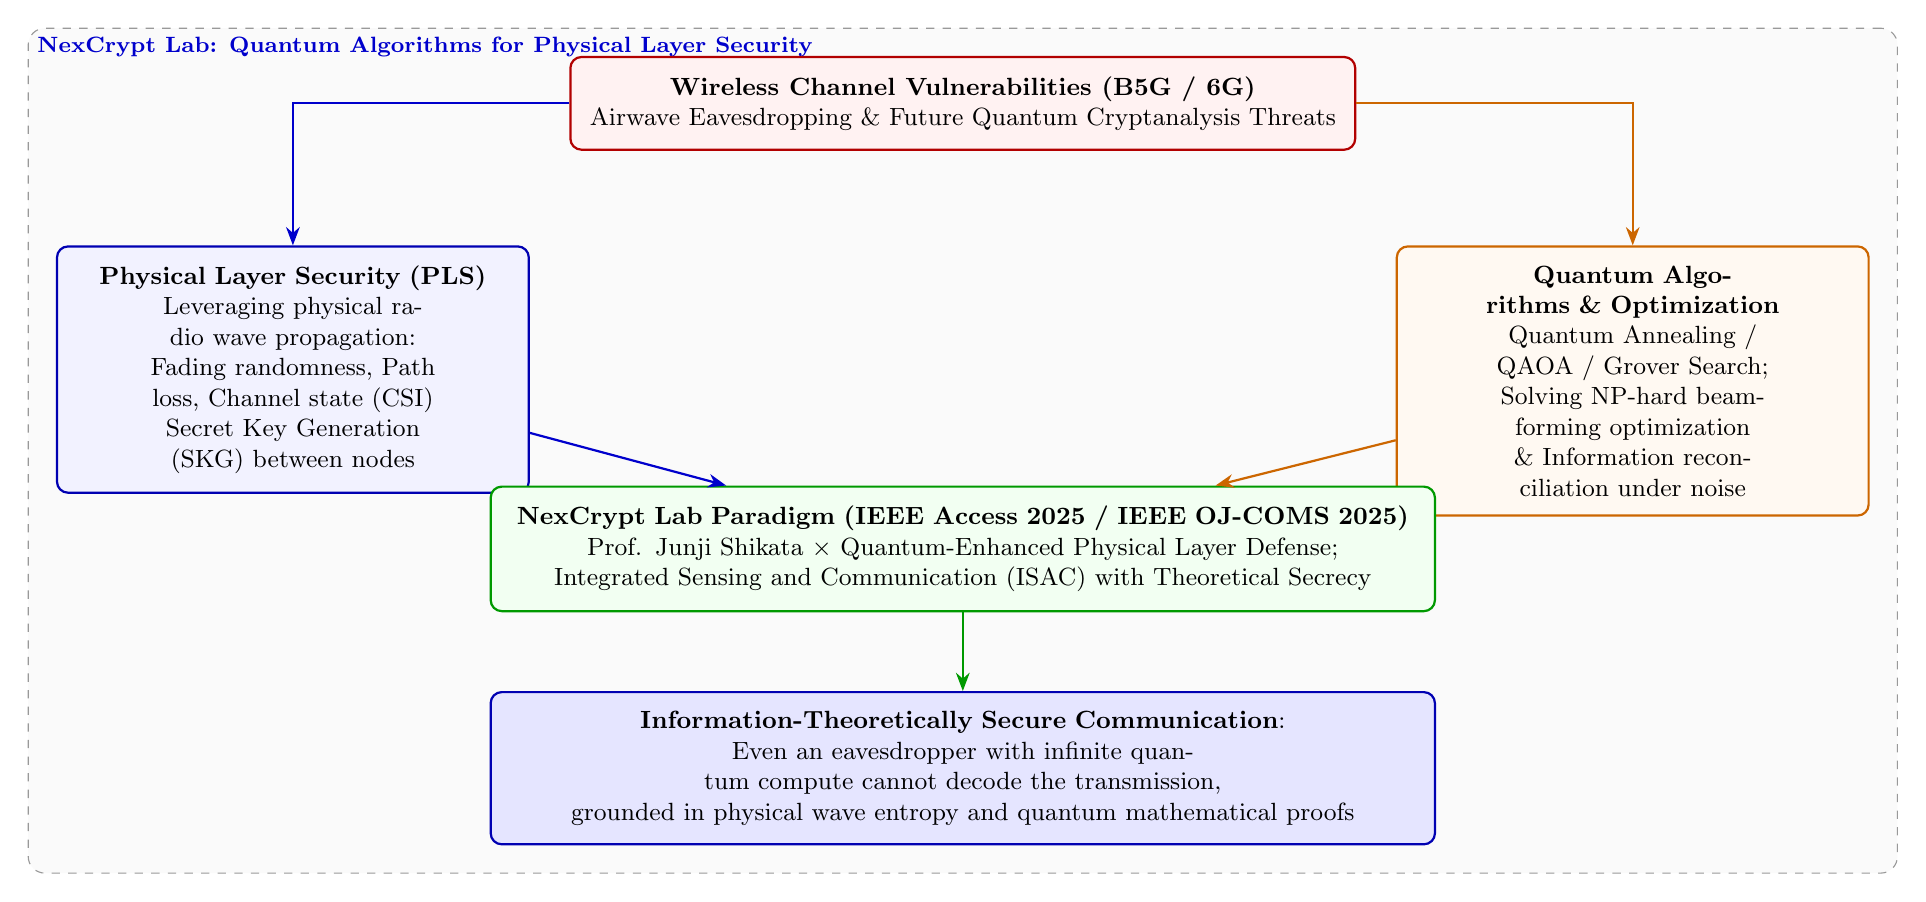
\begin{tikzpicture}[
    font=\small,
    >=Stealth,
    node distance=1.2cm,
    block/.style={rectangle, draw=blue!70!black, fill=blue!5, rounded corners=4pt, thick, align=center, inner sep=7pt},
    alertblock/.style={rectangle, draw=red!70!black, fill=red!5, rounded corners=4pt, thick, align=center, inner sep=7pt},
    greenblock/.style={rectangle, draw=green!60!black, fill=green!5, rounded corners=4pt, thick, align=center, inner sep=7pt},
    amberblock/.style={rectangle, draw=orange!80!black, fill=orange!5, rounded corners=4pt, thick, align=center, inner sep=7pt},
    groupbox/.style={draw=black!40, dashed, rounded corners=6pt, fill=black!2, inner sep=10pt}
]

    % Top Problem
    \node[alertblock] (wireless) {\textbf{Wireless Channel Vulnerabilities (B5G / 6G)}\\Airwave Eavesdropping \& Future Quantum Cryptanalysis Threats};

    % Two Pillars: PLS vs Quantum Algorithms
    \node[block, below left=1.2cm and 0.5cm of wireless, text width=5.5cm] (pls) {\textbf{Physical Layer Security (PLS)}\\Leveraging physical radio wave propagation:\\Fading randomness, Path loss, Channel state (CSI)\\Secret Key Generation (SKG) between nodes};

    \node[amberblock, below right=1.2cm and 0.5cm of wireless, text width=5.5cm] (quantum) {\textbf{Quantum Algorithms \& Optimization}\\Quantum Annealing / QAOA / Grover Search;\\Solving NP-hard beamforming optimization\\\& Information reconciliation under noise};

    \draw[->, thick, blue!80!black] (wireless) -| (pls);
    \draw[->, thick, orange!80!black] (wireless) -| (quantum);

    % Central Fusion: Prof. Shikata's Research
    \node[greenblock, below=1.4cm of $(pls)!0.5!(quantum)$, text width=11.5cm] (fusion) {\textbf{NexCrypt Lab Paradigm (IEEE Access 2025 / IEEE OJ-COMS 2025)}\\Prof. Junji Shikata $\times$ Quantum-Enhanced Physical Layer Defense;\\Integrated Sensing and Communication (ISAC) with Theoretical Secrecy};

    \draw[->, thick, blue!80!black] (pls) -- (fusion);
    \draw[->, thick, orange!80!black] (quantum) -- (fusion);

    % Bottom Result
    \node[block, fill=blue!10, below=1.0cm of fusion, text width=11.5cm] (result) {\textbf{Information-Theoretically Secure Communication}:\\Even an eavesdropper with infinite quantum compute cannot decode the transmission,\\grounded in physical wave entropy and quantum mathematical proofs};
    \draw[->, thick, green!60!black] (fusion) -- (result);

    \begin{scope}[on background layer]
        \node[groupbox, fit=(wireless) (pls) (quantum) (fusion) (result), label={[anchor=north west, font=\footnotesize\bfseries, blue!80!black]north west:NexCrypt Lab: Quantum Algorithms for Physical Layer Security}] {};
    \end{scope}

\end{tikzpicture}
\end{document}
